% Dr.DocBench Challenge 2026 -- technical report, team pranshu29
% Compile with the official ACL style files (acl.sty, acl_natbib.bst from https://github.com/acl-org/acl-style-files,
% or the ACL template on Overleaf): pdflatex paper && bibtex paper && pdflatex paper && pdflatex paper
\documentclass[11pt]{article}
\usepackage[final]{acl}
\usepackage{times}
\usepackage{latexsym}
\usepackage[T1]{fontenc}
\usepackage[utf8]{inputenc}
\usepackage{microtype}
\usepackage{inconsolata}
\usepackage{graphicx}
\usepackage{booktabs}
\usepackage{multirow}
\usepackage{amsmath}
\usepackage{xcolor}
\usepackage{url}
\usepackage{tikz}
\usetikzlibrary{positioning,arrows.meta,shapes.misc}
\usepackage{pgfplots}
\pgfplotsset{compat=1.17}

\newcommand{\ted}{Text\_ED}
\newcommand{\ro}{RO}
\newcommand{\up}[1]{\textcolor{green!45!black}{#1}}
\newcommand{\dn}[1]{\textcolor{red!65!black}{#1}}

\title{pranshu29 at Dr.DocBench 2026: Consensus Selection over\\Prompt-Diverse VLM Transcriptions for Expert-Level Document Parsing}

\author{Pranshu Rastogi \\
  Independent Researcher \\
  \texttt{rastogipranshu29@gmail.com} \And
  Rajneesh Tiwari \\
  Independent Researcher \\
  \texttt{rajneesh.vish1@gmail.com}}

\begin{document}
\maketitle

\begin{abstract}
We describe a training-free system for the Dr.DocBench document-parsing challenge, which asks for Markdown transcriptions of difficult book pages and scores text, reading order, display formulas and tables. One general vision-language model transcribes every page many times under different prompts, image settings and window sizes. A page-level minimum-Bayes-risk (MBR) selector, whose utility is the challenge's own text and reading-order matching, picks one transcription per page. Deterministic rules derived from a close reading of the evaluator refine it, and a gated word-level consensus layer fixes recognition slips that independent OCR engines confirm. Because display formulas and tables are scored by best match, the submission also carries LaTeX and HTML candidate blocks. The final system scored 84.54 overall on the 509 test pages (Text\_ED 0.1641, TEDS 71.86, CDM 81.84, reading order 85.65), rank 7. We document the full development path over 134 commits and more than 25 scored leaderboard submissions, ablate every component, quantify which development-set gains transferred to the hidden test set (selection changes: 68\%; convention rules: none), locate the remaining error with diagnostic submissions, and report a large set of measured negative results, including five stronger commercial models that did not beat the ensemble.
\end{abstract}

\section{Introduction}
This paper describes our system for the Dr.DocBench track of the DocInsights 2026 shared task \citep{docinsights2026}, held with the Workshop on Document Intelligence and Understanding at EMNLP 2026. The shared task has two tracks: DocSem, document-grounded quantitative reasoning with evidence attribution \citep{docsem}, and Dr.DocBench, expert-level parsing of complex document pages \citep{drdocbench, drdocbenchchallenge}; teams were ranked on the Dr.DocBench leaderboard hosted on EvalAI \citep{evalai}.

Dr.DocBench \citep{drdocbench} collects book pages on which current parsers disagree and annotates them with block-level references. The references follow conventions that vary from book to book: which lines form one block, whether text inside a picture is kept, whether a list is a table, and where running headers and page numbers sit in the reading order. A single strong model therefore loses points on pages it reads correctly.

We treat the task as selection under uncertainty rather than as model training. Our contributions are:
\begin{itemize}
  \setlength\itemsep{0pt}
  \item A pipeline that turns one vision-language model into a diverse candidate pool (prompts, preprocessing, windowing) and selects per page with MBR \citep{kumar-byrne-2004-minimum} using the official matching as the utility (\S\ref{sec:system}).
  \item Evaluator-aware rules (layout snapping, furniture merging, spill dropping, boundary voting) and a gated word-level consensus in the spirit of ROVER \citep{fiscus1997rover}, each validated by leave-one-out ablation (\S\ref{sec:ablations}).
  \item A step-by-step account of the development, with the leaderboard effect of every major change (\S\ref{sec:journey}), and an analysis of which development gains transferred to the test set and where the remaining error is (\S\ref{sec:analysis}).
  \item Measured negative results, including stronger commercial models used alone, as extra candidates, as proofreaders and as order sources (\S\ref{sec:negative}).
\end{itemize}

\section{Related Work}
\paragraph{Benchmarks.} Document-parsing benchmarks moved from layout detection, as in DocLayNet \citep{doclaynet} and M$^6$Doc \citep{m6doc}, to end-to-end page parsing with block-level annotations, as in OmniDocBench \citep{omnidocbench}, whose md2md scorer this challenge uses, and to OCR-centred evaluation of multimodal models in OCRBench v2 \citep{ocrbenchv2}. Dr.DocBench \citep{drdocbench} samples pages on which strong parsers disagree and adds expert content such as chemistry, music and dense formulas. Its metrics combine normalised edit distance \citep{levenshtein1966}, TEDS for tables \citep{teds} and CDM for formulas \citep{cdm}.

\paragraph{Parsing systems.} Pipeline toolkits combine layout detection with specialised recognisers: MinerU \citep{mineru}, PaddleOCR-VL \citep{paddleocrvl, paddleocrvl15} and Docling \citep{docling}. Compact end-to-end parsers include MinerU2.5 \citep{mineru25}, MinerU2.5-Pro \citep{mineru25pro}, DeepSeek-OCR 2 \citep{deepseekocr2} and GLM-OCR \citep{glmocr}. General vision-language models such as Kimi K2.5 \citep{kimik25} also transcribe pages when prompted, and the Dr.DocBench study found the strongest general models ahead of the specialised parsers on text and reading order \citep{drdocbench}.

\paragraph{Combining outputs.} Selecting among system outputs with minimum Bayes risk \citep{kumar-byrne-2004-minimum} and voting at the word level after alignment, as in ROVER \citep{fiscus1997rover}, are established in machine translation and speech recognition. We apply both to page transcriptions, using the challenge's matching as the utility and Hungarian assignment \citep{scipy} as implemented in the scorer.

\section{Task, Data and Evaluation}
\label{sec:task}
The development set has 986 pages from 66 books with Markdown and layout references; the test set has 509 pages from 34 books, five of whose subjects (Drama, Health \& Fitness, Juvenile Fiction, Nature, Travel) never occur in development. Each page is converted to Markdown and scored by the md2md pipeline of the official scorer, derived from OmniDocBench \citep{omnidocbench}. Text blocks are matched by normalised edit distance; \ted{} is the edit-distance ratio of matched blocks averaged over pages, and reading order (\ro) is one minus the normalised edit distance between the reference order of matched blocks and our order. Display formulas are scored with CDM \citep{cdm} and tables with TEDS \citep{teds}, each against its best-matching prediction. The overall score is the mean of the components available on a page, averaged over pages \citep{drdocbench}.

We ran the scorer locally on the development set and read its matcher in full. Four properties shaped the system:
\begin{enumerate}
  \setlength\itemsep{0pt}
  \item Consecutive predicted blocks are joined to match one reference block only if that block is at most 300 normalised characters and the page has at most 3600 reference$\times$prediction pairs. Above that, a segmentation mismatch cannot be repaired.
  \item Our unmatched blocks cost nothing while any reference block is unmatched; once every reference block is matched they are joined into one record and counted in full.
  \item Normalisation keeps only word characters (runs of four or more underscores become four), so punctuation and Markdown emphasis do not count, while case and digits do.
  \item Display formulas and tables do not take part in text or order matching, and unmatched predicted formulas and tables are ignored.
\end{enumerate}
A least-squares fit over 15 leaderboard rows gave Overall $\approx 0.558\,\mathrm{Text} + 0.433\,\mathrm{RO} + 0.054\,\mathrm{CDM} + 0.006\,\mathrm{TEDS} - 3.9$ (RMS residual 0.08), with $\mathrm{Text}=100\,(1-\text{\ted})$; we used it to plan uploads. Late in the challenge one CDM point was worth about 0.08 overall, so the fit understates formulas, and two table-only changes moved TEDS without moving Overall, so tables carry almost no weight on this test set.

\section{System}
\label{sec:system}

\begin{figure*}[t]
\centering
\resizebox{\textwidth}{!}{%
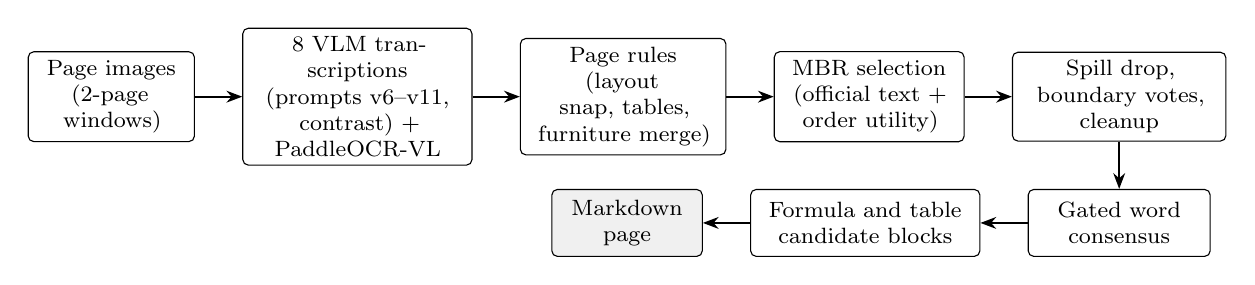
\begin{tikzpicture}[
  box/.style={draw, rounded corners=2pt, align=center, font=\footnotesize, inner sep=3pt, minimum height=8.5mm},
  arr/.style={-{Stealth[length=2mm]}, thick}]
\node[box, text width=19mm] (img) {Page images\\(2-page windows)};
\node[box, text width=27mm, right=6mm of img] (runs) {8 VLM transcriptions\\(prompts v6--v11,\\contrast) + PaddleOCR-VL};
\node[box, text width=24mm, right=6mm of runs] (rules) {Page rules\\(layout snap, tables,\\furniture merge)};
\node[box, text width=22mm, right=6mm of rules] (mbr) {MBR selection\\(official text +\\order utility)};
\node[box, text width=25mm, right=6mm of mbr] (post) {Spill drop,\\boundary votes,\\cleanup};
\node[box, text width=21mm, below=6mm of post] (cons) {Gated word\\consensus};
\node[box, text width=27mm, left=6mm of cons] (cand) {Formula and table\\candidate blocks};
\node[box, text width=17mm, left=6mm of cand, fill=black!6] (out) {Markdown\\page};
\draw[arr] (img) -- (runs); \draw[arr] (runs) -- (rules); \draw[arr] (rules) -- (mbr); \draw[arr] (mbr) -- (post);
\draw[arr] (post) -- (cons); \draw[arr] (cons) -- (cand); \draw[arr] (cand) -- (out);
\end{tikzpicture}}
\caption{System overview. Everything after the transcription runs is deterministic and training-free.}
\label{fig:pipeline}
\end{figure*}

Figure~\ref{fig:pipeline} shows the pipeline.

\subsection{Transcription runs}
The base model is a general vision-language model served free on OpenRouter during the challenge (\S\ref{sec:resources}). Pages are sent as two-page windows at 1600\,px on the long side with temperature 0. The prompt evolved through eleven versions; the ones in the final pool add these conventions:
\begin{itemize}
  \setlength\itemsep{0pt}
  \item \textbf{v6}: copy capitalisation exactly; never write placeholders for illegible text.
  \item \textbf{v7}: write page furniture (running header, footer, page number) after the body in a labelled section, because the references place it last.
  \item \textbf{v8}: a structural variant of v7 used as a third vote.
  \item \textbf{v10a/v10b/v11}: read multi-column pages column by column and start a new paragraph at a column break; v10b also splits paragraphs interrupted by pictures and keeps captions in their column's flow; v11 draws thin PaddleOCR-VL layout frames on the image.
\end{itemize}
Further runs vary contrast preprocessing, image size (1200\,px) and window size (one page); they serve as voters and pseudo-references. PaddleOCR-VL \citep{paddleocrvl} supplies layout blocks, furniture labels and tables, and the MinerU pipeline \citep{mineru} supplies formulas and independent word evidence.

\subsection{Page rules}
Every candidate passes through the same deterministic rules. \emph{Layout snap} splits our paragraphs at PaddleOCR-VL block boundaries where the text clearly spans two blocks (splits only, at most nine per page). \emph{Table add} inserts PaddleOCR-VL's table where the page has none. \emph{Furniture merge} joins the trailing header, footer and page-number lines that PaddleOCR-VL labels as furniture into one block: the references order furniture by hidden annotation order, and the matcher lists the positions of reference blocks folded into one of our blocks in reference order, so a merged block cannot be out of order.

\subsection{MBR selection}
For page $p$ with candidates $C$ and pseudo-references $R$, we pick
\begin{equation*}
\hat{c} = \arg\max_{c\in C} \frac{1}{|R_c|}\sum_{r\in R_c} \big(w_t\,T(c\,|\,r) + w_o\,O(c\,|\,r)\big),
\end{equation*}
where $R_c = R\setminus\{c\}$, $T(c\,|\,r)$ and $O(c\,|\,r)$ are the official text and reading-order scores of $c$ with $r$ standing in as the reference, and $(w_t,w_o)=(0.558,0.433)$. The final configuration (\emph{mbr8}) uses eight candidates (v6, v7, v8, the contrast run, PaddleOCR-VL, v10a, v10b, v11) and eleven pseudo-references (the five base runs and six column-break variants).

\subsection{Post-selection rules}
\emph{Spill drop} removes a paragraph that only the neighbouring page's one-page transcriptions contain (text that spilled across a two-page window). \emph{Boundary votes} split a long paragraph where at least five of eleven other runs split it; merges always hurt and are not applied. \emph{Cleanup} decodes HTML entities and strips inline tags.

\subsection{Gated word-level consensus}
Inside each body paragraph of the selected page, the matching paragraphs of the other runs (fuzzy match $\geq 90$) are aligned word by word. A word changes only when (i) a strict majority of all versions agrees, (ii) the new spelling is close to the old one (normalised similarity $\geq 0.75$) and not a case-only change, and (iii) an engine outside our model family confirms it: PaddleOCR-VL or MinerU has the new word and not the old one, or the old word is not a dictionary word. Insertions and deletions are limited to one word and never at a paragraph edge.

\subsection{Formula and table candidate blocks}
\label{sec:candidates}
Display formulas and tables are scored by best match and ignore unmatched predictions, and they take no part in text or order matching. The references write many styled lines (italic captions, bold labels, stage directions) as display formulas such as \texttt{\$\textbackslash textit\{\ldots\}\$}. The submission therefore carries, at the end of each page, standalone LaTeX candidates: each line of the page in the wrapper styles the references use (\texttt{\textbackslash textit}, \texttt{\textbackslash textbf}, bold italic, \texttt{\textbackslash text}, underlined), the corresponding lines of the other runs, and the inline formulas of all runs written as display formulas. Tables are handled the same way: alternative transcriptions from PaddleOCR-VL, crop-level transcriptions and other runs are included as additional HTML tables. These blocks leave the page's text and reading order unchanged; their effect on the formula score is traced in Table~\ref{tab:journey} and \S\ref{sec:ablations}.

\section{Development Journey}
\label{sec:journey}

\begin{figure}[t]
\centering
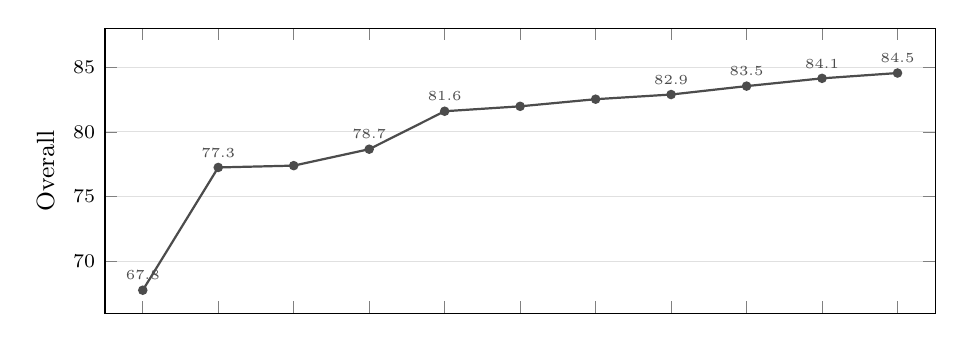
\begin{tikzpicture}
\begin{axis}[width=\columnwidth, height=5.2cm, ymin=66, ymax=88, xmin=0.5, xmax=11.5,
  xtick={1,...,11}, xticklabels={},
  ylabel={Overall}, ylabel style={font=\small}, tick label style={font=\scriptsize},
  ymajorgrids, grid style={black!12}, nodes near coords, point meta=explicit symbolic,
  every node near coord/.append style={font=\tiny, anchor=south}]
\addplot[thick, mark=*, mark size=1.3pt, black!70] coordinates {
 (1,67.77)[67.8] (2,77.25)[77.3] (3,77.39)[] (4,78.66)[78.7] (5,81.59)[81.6] (6,81.97)[] (7,82.52)[] (8,82.88)[82.9] (9,83.53)[83.5] (10,84.13)[84.1] (11,84.54)[84.5]};
\end{axis}
\end{tikzpicture}
\caption{Best leaderboard score after each kept change (steps 1--11 of Table~\ref{tab:journey}).}
\label{fig:journey}
\end{figure}

\begin{table*}[t]
\centering\small
\resizebox{\textwidth}{!}{%
\begin{tabular}{rllrrrrr}
\toprule
\# & Date & Change kept & \ted & TEDS & CDM & \ro & Overall \\
\midrule
1 & $\leq$09-26 & Single run, prompt v3 & -- & -- & -- & -- & 67.77 \\
2 & $\leq$09-26 & Furniture-last prompts v4--v7, medoid of four runs, layout snap & -- & -- & -- & -- & 77.25 \\
3 & $\leq$09-26 & PaddleOCR-VL tables where none & -- & 67.81 & -- & -- & 77.39 \\
4 & $\leq$09-26 & Contrast-preprocessed run as fifth vote & 0.1681 & 68.0 & 0 & 82.85 & 78.66 \\
5 & 09-27 & Italic formula candidates for short lines & 0.1681 & 68.0 & 55.0 & 82.85 & 81.59 \\
6 & 10-04 & More wrapper styles, formula pool, table candidates & 0.1681 & 71.86 & 63.21 & 82.85 & 81.97 \\
7 & 10-05 & Formula candidates from GPT-6.1 transcriptions of 120 pages & 0.1724 & 71.86 & 65.86 & 84.44 & 82.52 \\
8 & 10-05 & MBR selection, furniture merge, spill drop, boundary votes, cleanup & 0.1689 & 71.86 & 65.79 & 84.91 & 82.88 \\
9 & 10-06 & Formula candidates from all runs, symbol channel & 0.1689 & 71.86 & 76.54 & 84.91 & 83.53 \\
10 & 10-08 & Column-break runs as MBR candidates, word consensus & 0.1641 & 71.86 & 76.79 & 85.65 & 84.13 \\
\textbf{11} & 10-09 & \textbf{Final: more candidate sources and wrapper styles} & \textbf{0.1641} & \textbf{71.86} & \textbf{81.84} & \textbf{85.65} & \textbf{84.54} \\
\bottomrule
\end{tabular}}
\caption{Leaderboard results of the changes we kept, in order (dashes: component not recorded). Between steps 6 and 7 the leaderboard's evaluation changed, so compare steps 7--11 with each other.}
\label{tab:journey}
\end{table*}

Figure~\ref{fig:journey} and Table~\ref{tab:journey} trace the kept changes; Table~\ref{tab:failed} lists uploads that lost. The work fell into six phases.

\paragraph{Phase 1: one model, better prompts (67.8).} A harness sent two-page windows to the free model; the official scorer was wired in on day one. Moving page furniture to the end raised development \ro{} by about 12 points (the references never have body text after furniture), and explicit body/furniture sections (v7) added 1.7 \ro{} over v6.

\paragraph{Phase 2: ensemble and layout (77.3--78.7).} A medoid over three prompt variants and PaddleOCR-VL beat every single run (+1.04 over v7, best-of-four oracle 88.8 on development). Snapping our paragraphs to PaddleOCR-VL's block boundaries added +0.94; merging at those boundaries cost 1.15 and was dropped. A contrast-enhanced run as a fifth vote gained only +0.32 on development but +1.27 on test, whose pages have 28\% lower contrast.

\paragraph{Phase 3: formula and table candidates (81.6--82.5).} Formula scores were zero because our transcriptions contain almost no display formulas. Wrapping each short line as a standalone italic formula raised CDM from 0 to 55 without touching text or order; more wrapper styles, pooled formulas and alternative tables followed. A table crop pass (each PaddleOCR-VL table transcribed alone three times and voted) raised development TEDS from 70.0 to 77.0 but test TEDS by only 0.66 and Overall by $-0.01$.

\paragraph{Phase 4: the dev--test gap.} Three changes that improved development lost on test (Table~\ref{tab:failed}). We then located the test error by blanking groups of books (\S\ref{sec:analysis}) and found it concentrated in unseen-subject and high-disagreement books.

\paragraph{Phase 5: metric-aware selection (82.9--83.5).} MBR with the official matching as utility replaced the medoid (+1.19 on development; +1.84 with the furniture merge), followed by spill drop, boundary votes and cleanup. A same-day comparison credits this stack with +0.36 on test (\ted{} $-0.0035$, \ro{} $+0.47$).

\paragraph{Phase 6: column-break runs and consensus (84.1--84.5).} Prompts v10a/v10b/v11 encode the references' column-break convention. Imported as paragraph splits they helped development (+1.00 per page) but cost test text, because most of the gain came from splits inside list blocks, a development-book convention. Used instead as MBR candidates and pseudo-references (\emph{mbr8}), they gave +0.60 on test (\ted{} $-0.0048$, \ro{} $+0.74$). The gated word consensus and a final round of formula candidates brought the score to 84.54.

\begin{table}[t]
\centering\small
\setlength{\tabcolsep}{4pt}
\begin{tabular}{lrr}
\toprule
Upload & Dev & Test \\
\midrule
Contrast runs as extra votes & \up{+0.39} & \dn{$-$0.84} \\
One-page windows as the pool & \up{+1.02} & \dn{$-$0.63} \\
GPT-6.1 sol-pro on 120 hard pages & \up{+0.06} & \dn{$-$0.47} \\
Drop text PaddleOCR-VL lacks & \up{+0.02} & \dn{$-$0.21} \\
Column splits incl.\ list splits & \up{+1.00} & \dn{$-$0.02} \\
Index-entry splits & \up{+0.08} & \dn{$-$0.02} \\
End-to-end-tuned formula pools & \up{+1.09} & \dn{$-$3.00} \\
\bottomrule
\end{tabular}
\caption{Uploads that lost on the leaderboard although they improved development (Overall, leaderboard units). The last row tested, and refuted, the hypothesis that the leaderboard scores with the end-to-end (layout JSON) pipeline: removing wrapper candidates left \ro{} at exactly 84.91 and dropped CDM from 65.8 to 12.5.}
\label{tab:failed}
\end{table}

\section{Ablations}
\label{sec:ablations}

\paragraph{Rules.} Table~\ref{tab:loo} removes each rule from the final pipeline on 925 development pages. Every rule helps; the layout rules matter most.

\begin{table}[t]
\centering\small
\setlength{\tabcolsep}{4pt}
\begin{tabular}{lrrr}
\toprule
Pipeline & \ted & \ro & $\Delta$ \\
\midrule
Final (mbr8 + rules) & 0.1168 & 88.58 & -- \\
\quad -- layout snap and tables & 0.1204 & 87.11 & \dn{$-$0.84} \\
\quad -- furniture merge & 0.1162 & 87.49 & \dn{$-$0.44} \\
\quad -- boundary votes & 0.1186 & 88.48 & \dn{$-$0.14} \\
\quad -- spill drop & 0.1187 & 88.55 & \dn{$-$0.12} \\
\quad -- cleanup & 0.1169 & 88.58 & \dn{$-$0.01} \\
\quad + gated word consensus & 0.1168 & 88.58 & \up{+0.005} \\
\bottomrule
\end{tabular}
\caption{Leave-one-out on 925 development pages ($\Delta$ in leaderboard units, $0.558\,\mathrm{Text}+0.433\,\mathrm{RO}$; book-clustered bootstrap: the intervals for layout snap and boundary votes exclude zero).}
\label{tab:loo}
\end{table}

\paragraph{Selection.} Over the same rule stack, MBR beat the medoid by +1.05 on development (book-clustered CI $[+0.38,+1.85]$). Weighted MBR, ridge and gradient-boosting rankers over 16--21 label-free features, and paragraph-level fusion were all within noise of plain MBR; picking the best of the same five runs per page (an oracle) would add +4.8 over the medoid, so selection, not reading, limits us. Adding the six column-break variants as pseudo-references gave +0.36; adding v10a/v10b/v11 as candidates gave +0.88 (\ted{} 0.1264$\to$0.1168, \ro{} 87.79$\to$88.58). Using all 17 runs as references diluted the column-break signal (+0.59). Weighting the utility towards text (0.7/0.3) traded order for text (+0.15).

\paragraph{Segmentation.} Column-break split import from the v10 runs: when at least two of three runs split, all kinds of breaks +0.08 on development and $-0.02$ on test; without splits inside one layout block $-0.005$; any one of three runs \ro{} $+0.27$ but \ted{} $+0.0033$.

\paragraph{Word consensus.} A plain majority vote lost 0.06 (32 pages worse, 6 better): our runs share one model and its errors, and runs that split a paragraph differently vote to delete phrases at its edges. Restricting votes to near-spellings, away from edges and confirmed by an independent engine removes every regression (+0.006, one page better, none worse); on test it changes 33 words on 24 pages, mostly real OCR slips (\emph{ATHAWAY}$\to$\emph{HATHAWAY}, \emph{Macmillian}$\to$\emph{Macmillan}, Polish diacritics).

\paragraph{Formula candidates.} On the leaderboard, CDM rose with the number of candidate forms offered: 0 without candidates, 55.0 with italic candidates for short lines, 63.2 adding bold and bold-italic styles, longer lines and pooled formulas, 65.9 adding candidates from a second model's transcriptions of 120 pages, 76.5 with candidates from every run, and 81.8 with more runs and plain and underlined styles. Text and order were byte-identical across these steps.

\section{Analysis}
\label{sec:analysis}

\subsection{What transferred to the test set}
Selection changes transferred: mbr8 kept 68\% of its development gain overall, 94\% for \ro{} and about 50\% for text. Changes that touched most pages or that encode a development-book convention reversed (Table~\ref{tab:failed}). Dev overstated the absolute test score of a single run by 4.5 points.

\subsection{Locating the test error}
Three diagnostic submissions blanked groups of test books; the change in leaderboard \ted{} and \ro{} gives each group's own scores (Table~\ref{tab:probe}). The 240 pages of unseen-subject and high-disagreement books held 56\% of the text error and most of the order error; bringing them to the level of the rest would be worth about +2.4 overall, the gap to the top team of the time.

\begin{table}[t]
\centering\small
\setlength{\tabcolsep}{3.5pt}
\begin{tabular}{lrrr}
\toprule
Test books & Pages & \ted & \ro \\
\midrule
G1: subjects absent from dev & 120 & 0.200 & 77.4 \\
G2: highest run disagreement & 120 & 0.203 & 80.7 \\
G3: half of the rest & 134 & 0.157 & 85.0 \\
G4: other half (derived) & 135 & 0.120 & 87.5 \\
\bottomrule
\end{tabular}
\caption{Per-group test scores decoded from blanking submissions (pipeline of step 5).}
\label{tab:probe}
\end{table}

\subsection{Where the text error is}
On development, the final pipeline's text error splits into matched blocks with edits (49\%), our text that no reference block contains (40\%), and missing reference text (11\%); letter edits inside matched blocks are 42\% of all text error, digit edits 6\% and case-only edits 1\%. Half of all text error sits on 8\% of the pages, where the reference made a book-specific choice: picture text kept as an image, a directory kept as a table, crossword clues kept as one long block, a page whose reference is only its page number. Our words on those pages are right; the choice is visible neither in the image nor in our runs.

\subsection{Where the order error is}
Of 11.4 development \ro{} points lost, displaced body blocks account for 3.74, unmatched body blocks (segmentation) 1.83, titles 1.31, page numbers 1.21, running headers 0.96 and captions 1.02. The references order the page-end furniture by annotation order (header before page number and the reverse occur within one book), which the furniture merge neutralises only when PaddleOCR-VL labels the lines; merging unlabelled tail lines cost 0.08--0.62. The worst pages are catalogues, labelled diagrams, crosswords and verse, each with its own convention.

\section{Negative Results}
\label{sec:negative}

\begin{table}[t]
\centering\small
\setlength{\tabcolsep}{3pt}
\begin{tabular}{lrrr}
\toprule
Model (53 common dev pages) & \ted & \ro & $\Delta$ \\
\midrule
Our pipeline (mbr8) & 0.0857 & 88.45 & -- \\
Free model v7 alone & 0.0818 & 86.11 & $-$0.79 \\
Kimi K2.5 (OpenRouter) & 0.0614 & 85.20 & $-$0.05 \\
Kimi K2.5 (HF, other host) & 0.0926 & 79.65 & $-$4.19 \\
Gemini 3.8 Flash & 0.0682 & 84.90 & $-$0.56 \\
Kimi K2.6, no thinking & 0.1053 & 83.71 & $-$3.14 \\
\midrule
GPT-6 sol-pro (897 pages) & 0.1380 & 83.69 & $-$3.19 \\
\bottomrule
\end{tabular}
\caption{Single models against the ensemble on development. As extra MBR candidates they add +0.1 to +0.2 once one outlier page is removed; Kimi K2.5 inside mbr8: $-0.02$.}
\label{tab:models}
\end{table}

Table~\ref{tab:models} compares stronger models. Kimi K2.5 reads text best but orders worse; the same model behind a different inference host scored 4.1 points lower. Further attempts that did not help:
\begin{itemize}
  \setlength\itemsep{0pt}
  \item Another model's paragraph order applied to our text: $-1.07$ (GPT-6 sol-pro), $-1.32$ (GPT-6.1), $-1.34$ (Kimi).
  \item Proofreading our page with Kimi K2.5 given the image: $-2.6$ as returned (it re-split paragraphs); word-level fixes only $\pm 0.00$, 13 edits in 37 pages.
  \item Paragraph boundaries from PaddleOCR-VL or MinerU, also only on high-disagreement books: $-1.4$ to $-1.7$.
  \item Geometric column-major reordering ($-3.2$ to $-4.5$ \ro), consensus order ($-1.08$ \ro), moving running heads ($-0.2$ to $-0.3$ per page), merging short paragraphs ($-0.6$ to $-1.1$), list chunking under the 300-character limit ($-0.8$ to $-1.8$).
  \item Writing styled lines once as LaTeX in place of Markdown emphasis: $-0.6$ to $-2.2$ on development, where references keep 279 styled blocks as Markdown and 39 as LaTeX.
  \item Claude Sonnet refused to transcribe copyrighted book pages; MiMo v2.6 Pro, GLM and DeepSeek vision models were 6--9 points below the free model.
\end{itemize}

\section{Resources and Disclosure}
\label{sec:resources}
Table~\ref{tab:resources} lists every model and tool we ran. Models were called through OpenRouter \citep{openrouter} and Hugging Face Inference Providers \citep{hfinference}; layout and OCR toolkits ran on Kaggle GPUs; string matching used RapidFuzz \citep{rapidfuzz} and the official scorer.
\begin{itemize}
  \setlength\itemsep{0pt}
  \item \textbf{Base model}: an unnamed vision-language model offered free on OpenRouter during the challenge \citep{stealthmodel}; every transcription in the final candidate pool comes from it.
  \item \textbf{Also in the final submission}: GPT-6.1 sol-pro transcriptions of 120 test pages, used only as a source of formula and table candidates.
  \item \textbf{Training and data}: none. No fine-tuning, no external annotated data, no manual edits to test output. The official scorer was run locally on the development set only.
  \item \textbf{Leaderboard use}: more than 25 scored submissions, of which three blanked groups of books to locate error and several applied one change to one group of books to measure it there.
  \item \textbf{Formula and table candidate blocks}: described in \S\ref{sec:candidates}.
  \item \textbf{Cost}: about \$82 of API usage in total, all models.
\end{itemize}

\begin{table*}[t]
\centering\footnotesize
\setlength{\tabcolsep}{4pt}
\resizebox{\textwidth}{!}{%
\begin{tabular}{@{}lllp{2.5cm}p{4.3cm}p{2.9cm}@{}}
\toprule
Model or tool & Developer & Weights & Access & Role & Ref. \\
\midrule
space-bunny-alpha (stealth) & not disclosed & -- & OpenRouter (free) & base transcriber, all candidates & \citealp{stealthmodel} \\
PaddleOCR-VL (pipeline 1.6) & Baidu & open & Kaggle GPU & layout, furniture labels, tables, formulas & \citealp{paddleocrvl, paddleocrvl15} \\
MinerU (pipeline 2.7.6) & OpenDataLab & open & Kaggle GPU & formulas, word evidence for consensus & \citealp{mineru} \\
Docling & IBM Research & open & Kaggle GPU & picture boxes for analysis & \citealp{docling} \\
GPT-6.1 sol-pro & OpenAI & closed & OpenRouter & formula and table candidates (120 test pages) & \citealp{gpt61solpro} \\
GPT-6 sol-pro & OpenAI & closed & OpenRouter (batch) & tested: reader, order source & \citealp{gpt6solpro} \\
GPT-6 luna-pro & OpenAI & closed & OpenRouter & tested: reader & \citealp{gpt6lunapro} \\
Gemini 3.8 Flash & Google & closed & OpenRouter & tested: reader, MBR candidate & \citealp{gemini38flash} \\
Claude Sonnet 5.5 & Anthropic & closed & OpenRouter (batch) & tested: declined copyrighted pages & \citealp{claudesonnet55} \\
Kimi K2.5 & Moonshot AI & open & OpenRouter, HF Inference & tested: reader, candidate, proofreader & \citealp{kimik25} \\
Kimi K2.6 & Moonshot AI & open & HF Inference & tested: reader, candidate & \citealp{kimik26} \\
Qwen3.8 Flash & Alibaba Qwen & -- & OpenRouter & tested: extra ensemble vote & \citealp{qwen38} \\
Qwen3.8 27B & Alibaba Qwen & open & OpenRouter (free) & tested: rate-limited, dropped & \citealp{qwen38} \\
GLM-5.3 Flash & Z.ai (Zhipu) & -- & OpenRouter (batch) & tested: reader & \citealp{glm53flash} \\
DeepSeek V4.1 Flash & DeepSeek & -- & OpenRouter (batch) & tested: reader & \citealp{deepseekv41} \\
MiMo v2.6 Pro & Xiaomi & -- & OpenRouter & tested: reader & \citealp{mimo26pro} \\
dots-3-note-preview & dots studio & -- & OpenRouter (free) & tested: reader & \citealp{dots3note} \\
\bottomrule
\end{tabular}}
\caption{Every model and tool used. Weights: open (public weights or open-source code), closed, or -- (served through an API; we did not check whether weights are public). ``Tested'' means evaluated on the development set and not used in the final submission (\S\ref{sec:negative}).}
\label{tab:resources}
\end{table*}

\section*{Limitations}
The system depends on a free model that was withdrawn during the challenge, so the transcriptions cannot be regenerated; we archived all candidate outputs. All candidates come from one model family, which caps what consensus can fix: the oracle over our five base runs is 3.7 points above MBR, but most of that gap lies on pages where every run follows the same wrong convention. The formula and table scores rely on the candidate blocks of \S\ref{sec:candidates}, which the metrics evaluate by best match. The development set shares no books with the test set, so convention-level rules were tuned on books whose annotators made different choices.

\section*{Ethics Statement}
The pages are from copyrighted books. We do not release transcriptions of the development or test pages; the public repository contains code, prompts, logs and aggregate results only. We did not prompt models to bypass refusals. Diagnostic leaderboard submissions measured groups of books, not individual pages or lines.

\section{Conclusion}
A single capable model, prompted several ways and filtered by MBR with the evaluation metric as utility, beat every stronger model we could access on this benchmark. Selection changes transferred to the hidden test set; rules tuned to development-book conventions did not. The remaining gap to the leading teams, about 0.025 \ted{} and 4 \ro{} points, lies in segmentation and reading-order conventions that vary by book, which a layout-aware model trained on the annotation guidelines could address.

\bibliography{references}

\appendix

\section{Prompt Excerpts}
\label{app:prompts}
\paragraph{Furniture section (v7 onwards).} \emph{``Page furniture (running headers, running footers, page numbers, publisher lines, book or chapter titles repeated at the top or bottom of the page, copyright notices) is transcribed too, but it is always written AFTER the body of that page, never where it is printed\ldots{} first the line {<}{<}{<}BODY{>}{>}{>} followed by all body content in reading order\ldots{} then the line {<}{<}{<}FURNITURE{>}{>}{>} followed by the page furniture.''}

\paragraph{Column breaks (v10a).} \emph{``Read each column completely from top to bottom before moving to the next column (left to right). A heading, picture or table that spans the full page width ends one band of columns\ldots{} When a paragraph runs from the bottom of one column into the top of the next column, end it at the column break and write the continuation as a NEW paragraph.''}

\section{Tools}
\label{app:tools}
The repository contains the harness (\texttt{predict.py}), the deterministic builder that rebuilds every uploaded file byte-identically from archived candidates (\texttt{stack.py}, \texttt{build\_submission.py}), the MBR selector (\texttt{mbr\_refs\_choose.py}), the consensus layer (\texttt{rover.py}), the ablation and bootstrap tools (\texttt{ablate.py}, \texttt{ablate\_vs.py}), the leaderboard decoders (\texttt{probe\_decode.py}, \texttt{lb\_decode.py}), and the analyses behind \S\ref{sec:analysis} (\texttt{text\_anatomy2.py}, \texttt{ro\_anatomy3.py}). \texttt{MILESTONES.md} and \texttt{SUBMISSIONS.md} summarise the experiments and the leaderboard submissions.

\end{document}
